

% \documentclass[12pt]{extarticle}
% \usepackage{geometry}


% \usepackage{scicite}
% \usepackage{fixltx2e}
% \usepackage{mathtools}
% \usepackage{graphicx}
% \usepackage{hyperref}
% \usepackage{colortbl}
% \usepackage{xcolor}
% \usepackage{booktabs}
% \usepackage{tikz}
% \usepackage{pgfplots}




% \usepackage{times}



% \topmargin 2.0cm
% \oddsidemargin 0.2cm
% \textwidth 16cm 
% \textheight 21cm
% \footskip 1.0cm

% \renewcommand{\baselinestretch}{0.5} 


% \newenvironment{sciabstract}{%
% \begin{quote} \bf}
% {\end{quote}}



% \renewcommand\refname{References and Notes}


% \newcounter{lastnote}
% \newenvironment{scilastnote}{%
% \setcounter{lastnote}{\value{enumiv}}%
% \addtocounter{lastnote}{+1}%
% \begin{list}%
% {\arabic{lastnote}.}
% {\setlength{\leftmargin}{.22in}}
% {\setlength{\labelsep}{.5em}}}
% {\end{list}}



\documentclass[12pt]{article}


\usepackage{scicite}
\usepackage{fixltx2e}
\usepackage{mathtools}
\usepackage{graphicx}



\usepackage{times}



\topmargin 0.0cm
\oddsidemargin 0.2cm
\textwidth 16cm 
\textheight 21cm
\footskip 1.0cm

\renewcommand{\baselinestretch}{0.5} 


\newenvironment{sciabstract}{%
\begin{quote} \bf}
{\end{quote}}



\renewcommand\refname{References and Notes}


\newcounter{lastnote}
\newenvironment{scilastnote}{%
\setcounter{lastnote}{\value{enumiv}}%
\addtocounter{lastnote}{+1}%
\begin{list}%
{\arabic{lastnote}.}
{\setlength{\leftmargin}{.22in}}
{\setlength{\labelsep}{.5em}}}
{\end{list}}




\title{{\it \textbf{Experiment 2:\hspace{0.5cm} Design of common source amplifier}\/} } 




\author
{Satyanand 14EC10049\\
\normalize{Rohit Kumar 14EC10043}
}


\date{}






\begin{document} 

% Double-space the manuscript.

%spacing between lines
\baselineskip14pt

% Make the title.

%\maketitle 








\renewcommand{\baselinestretch}{0.5} 

\section*{Objective}
%\vspace{-\baselineskip}
\begin{itemize}
    \item Familiarization with Input-Output I-V relationship of MOS transistors through measured characteristic data.
    \item To know practical values of device model parameters
\end{itemize}

% To study the DC characteristics of a MOSFET and to
% observe the relation between V\_G\_S versus I\_D and 
% V\textsubscript{GS} versus I\_D and to obtain large signal parameters(V\_D,V\_t,$\lambda$,
% \textit{t})

\section*{Components}
\begin{itemize}
    \item MOSFET
    \item Breadboard%
    \item Resistors 1k$\Omega$
    \item Potentiometers 10k$\Omega$ and  4k$\Omega$  range
    \item Connecting wires
\end{itemize}

\section*{Circuit Diagram}
%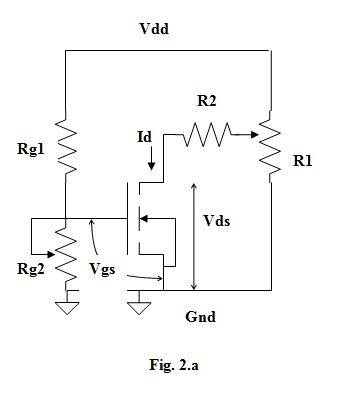
\includegraphics{ckt.jpg}
 % \caption{Circuit diagram}
  %\label{fig:boat1}
  
%\section*{Design Steps:}

\section*{Observation Table}
% \subsection{Id versus V\_D\_S for Vgs=5.95V}
% \begin{tikzpicture}
%   \begin{axis}[
%     xlabel=Cost,
%     ylabel=Error,
%     height=9cm,
%     width=17cm,   
%     grid=major,]
    
%   %\addplot {-x^5 - 242};
%   %\addlegendentry{model}

%   \addplot coordinates {
%     ( 0 , 12.06 )
%     ( 1.33 , 12.07 )
%     ( 1.74 , 12.06 )
%     ( 2.27 , 11.58 )
%     ( 2.31 , 11.4 )
%     ( 2.42 , 11.13 )
%     ( 2.54 , 10.86 )
%     ( 2.67 , 10.48 )
%     ( 2.83 , 9.95 )
%     ( 3.03 , 9.15 )
%     ( 3.19 , 8.5 )
%     ( 3.27 , 8.07 )
%     ( 3.45 , 7.39 )
%     ( 3.56 , 6.86 )
%     ( 3.68 , 6.18 )
%     ( 3.8 , 5.53 )
%     ( 3.81 , 5.37 )
%     ( 3.86 , 5.1 )
%     ( 3.94 , 4.78 )
%     ( 4.07 , 3.89 )
%     ( 4.11 , 3.63 )
%     ( 4.19 , 3.13 )
%     ( 4.29 , 2.48 )
%     ( 4.35 , 2.16 )
%     ( 4.57 , 1.29 )
%     ( 4.73 , 1.1 )
%     ( 4.93 , 0.96 )
%     ( 5.42 , 0.78 )
%     ( 5.69 , 0.72 )
%     ( 6.15 , 0.64 )
%     ( 7.63 , 0.5 )
%     ( 10.14 , 0.4 )
%     ( 11.2 , 0.36 )
    
     
    
%   };
%   \legend{Case 1}
%   %\addlegendentry{estimate}
%   \end{axis}
% \end{tikzpicture}


\subsection{Id versus V$_D_S$ for Vgs=7.8V}
\begin{center}
 \begin{tabular}{|| c | c||} 
 \hline
 Vds(V) & Id(mA) \\ [0.5ex] 
 \hline\hline
 1.53 & 12.02 \\
\hline
1.78 & 12.01 \\
\hline
1.97 & 11.83 \\
\hline
2.14 & 11.54 \\
\hline
2.24 & 11.29 \\
\hline
2.31 & 11.05 \\
\hline
2.36 & 10.88 \\
\hline
2.45 & 10.54 \\
\hline
2.55 & 10.13 \\
\hline
2.63 & 9.78 \\
\hline
2.7 & 9.38 \\
\hline
2.77 & 9.04 \\
\hline
2.81 & 8.86 \\
\hline
2.87 & 8.57 \\
\hline
2.91 & 8.19 \\
\hline
2.98 & 7.81 \\
\hline
3 & 7.67 \\
\hline
3.06 & 7.27 \\
\hline
3.11 & 6.98 \\
\hline
3.17 & 6.55 \\
\hline
3.22 & 6.14 \\
\hline
3.3 & 5.64 \\
\hline
3.4 & 4.99 \\
\hline
3.43 & 4.57 \\
\hline
3.51 & 4.11 \\
\hline
3.61 & 3.83 \\
\hline
3.59 & 3.46 \\
\hline
3.64 & 2.94 \\
\hline
3.69 & 2.6 \\
\hline
3.74 & 2.08 \\
\hline
3.78 & 1.7 \\
\hline
3.85 & 1.22 \\
\hline
3.94 & 0.99 \\
\hline
4.1 & 0.8 \\
\hline
4.88 & 0.54 \\
\hline
5.86 & 0.41 \\
\hline
6.3 & 0.38 \\
\hline


\end{tabular}
\end{center}

\subsection{Id versus V$_D_S$ for Vgs=9.7V}
\begin{center}
 \begin{tabular}{|| c | c||} 
 \hline
 Vds(V) & Id(mA) \\ [0.5ex] 
 \hline\hline
 0.0 & 12.06 \\
\hline
1.33 & 12.07 \\
\hline
1.74 & 12.06 \\
\hline
2.27 & 11.58 \\
\hline
2.31 & 11.4 \\
\hline
2.42 & 11.13 \\
\hline
2.54 & 10.86 \\
\hline
2.67 & 10.48 \\
\hline
2.83 & 9.95 \\
\hline
3.03 & 9.15 \\
\hline
3.19 & 8.5 \\
\hline
3.27 & 8.07 \\
\hline
3.45 & 7.39 \\
\hline
3.56 & 6.86 \\
\hline
3.68 & 6.18 \\
\hline
3.8 & 5.53 \\
\hline
3.81 & 5.37 \\
\hline
3.86 & 5.1 \\
\hline
3.94 & 4.78 \\
\hline
4.07 & 3.89 \\
\hline
4.11 & 3.63 \\
\hline
4.19 & 3.13 \\
\hline
4.29 & 2.48 \\
\hline
4.35 & 2.16 \\
\hline
4.57 & 1.29 \\
\hline
4.73 & 1.1 \\
\hline
4.93 & 0.96 \\
\hline
5.42 & 0.78 \\
\hline
5.69 & 0.72 \\
\hline
6.15 & 0.64 \\
\hline
7.63 & 0.5 \\
\hline
10.14 & 0.4 \\
\hline
11.2 & 0.36 \\
\hline

\end{tabular}
\end{center}

\subsection{Id versus V$_G_S$ for Vds=6V}
\begin{center}
 \begin{tabular}{|| c | c||} 
 \hline
 Vds(V) & Id(mA) \\ [0.5ex] 
 \hline\hline
 1.74 & 12.04 \\
\hline
1.88 & 11.9 \\
\hline
2.0 & 11.63 \\
\hline
2.14 & 11.13 \\
\hline
2.23 & 10.69 \\
\hline
2.28 & 10.38 \\
\hline
2.37 & 9.79 \\
\hline
2.44 & 9.29 \\
\hline
2.51 & 8.71 \\
\hline
2.58 & 8.13 \\
\hline
2.61 & 7.87 \\
\hline
2.65 & 7.52 \\
\hline
2.68 & 7.18 \\
\hline
2.74 & 6.55 \\
\hline
2.78 & 6.17 \\
\hline
2.82 & 5.69 \\
\hline
2.86 & 5.27 \\
\hline
2.88 & 5.0 \\
\hline
2.91 & 4.68 \\
\hline
2.95 & 4.17 \\
\hline
2.98 & 3.78 \\
\hline
3.03 & 3.25 \\
\hline
3.08 & 2.52 \\
\hline
3.12 & 2.09 \\
\hline
3.36 & 0.58 \\
\hline
4.17 & 0.31 \\
\hline
4.45 & 0.28 \\
\hline
4.83 & 0.25 \\
\hline
5.61 & 0.2 \\
\hline

 


\end{tabular}
\end{center}
 
 
 

\section*{Plots}

\subsection*{Plot of V_O_U_T vs V_I_N}
\begin{center}
    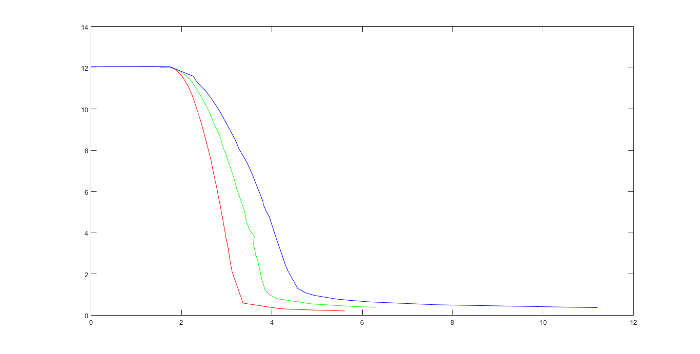
\includegraphics{data.png}
\end{center}

\subsection*{Gain versus }
\begin{center}
    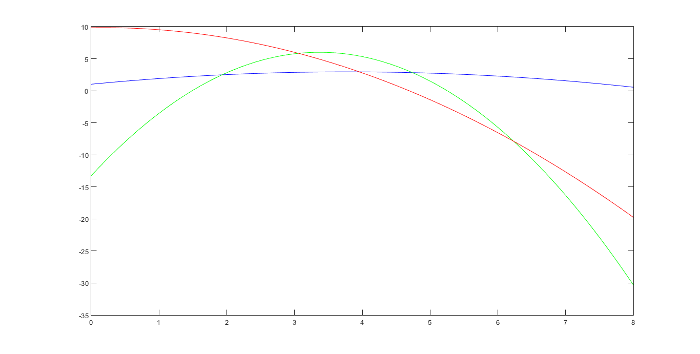
\includegraphics{gain.png}
\end{center}

\subsection*{Gain versus }
\begin{center}
    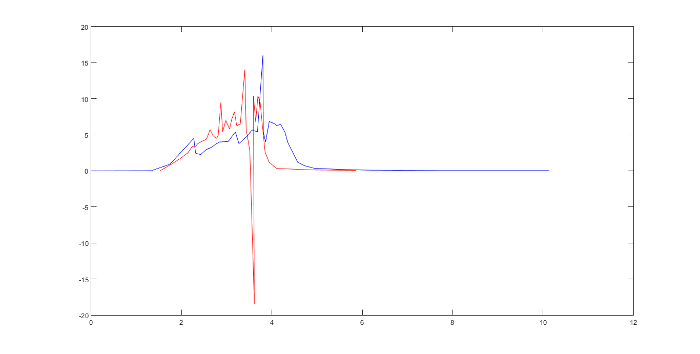
\includegraphics{gain_data.png}
\end{center}

\subsection*{Gain versus }
\begin{center}
    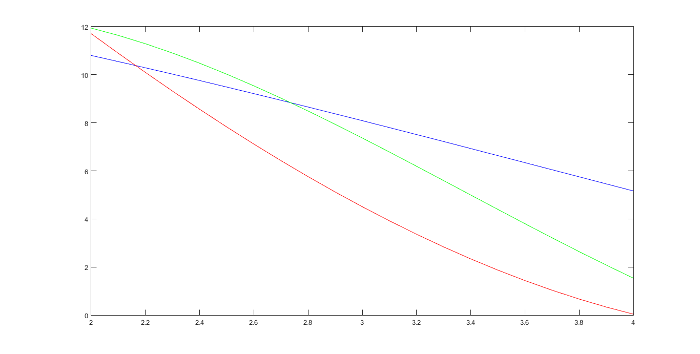
\includegraphics{linear_poly.png}
\end{center}

\subsection*{Gain versus }
\begin{center}
    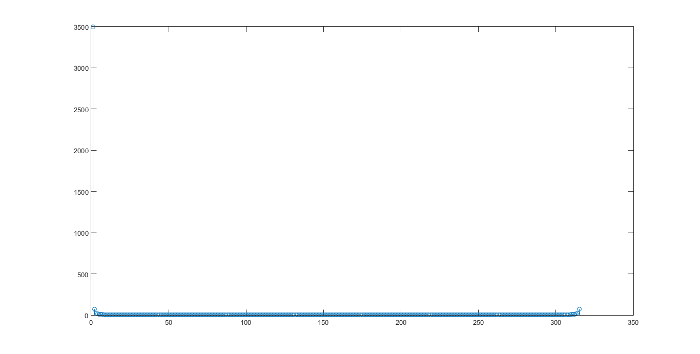
\includegraphics{stem1.png}
\end{center}

\subsection*{Gain versus }
\begin{center}
    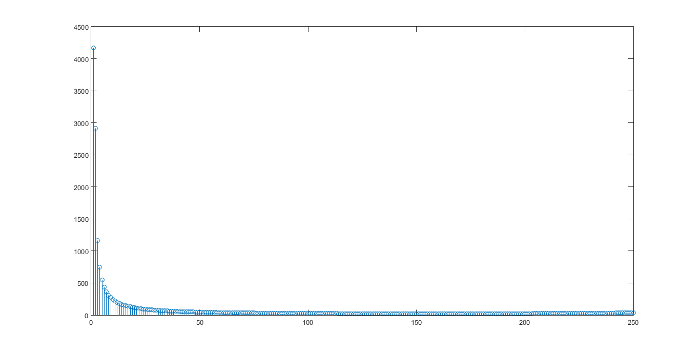
\includegraphics{stem2.png}
\end{center}

\subsection*{Gain versus }
\begin{center}
    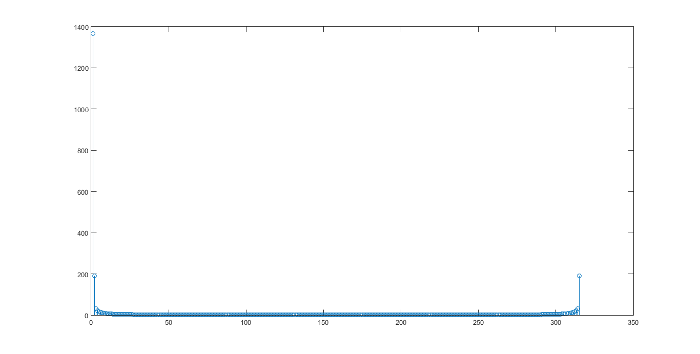
\includegraphics{stem3.png}
\end{center}

\section*{Results}

\subsection*{THD values for }
\begin{center}
 \begin{tabular}{|| c | c| c ||}
 \hline
 \hline
 K_1^2 & \lambda(V^-^1) & g_d(mS) \\
 \hline\hline\\
 -9.59 & 0.104 & 0.72\\
 \hline
 -220.49 & 4.5x10^-^3 & 9.4x10^-^3\\
 \hline
 -358.19 & 2.79x10^-^3 & 0.017\\
 \hline
\end{tabular}
\end{center}
 
\subsection*{Large signal parameters from Id vs Vds plot}

\begin{center}
 \begin{tabular}{|| c | c| c ||}
 \hline
 \hline
 V_t_h(V) & k & g_m(m\Omega) \\
 \hline\hline
  4.14 & 2.25 & 2.25\\
  \hline
 


\end{tabular}
\end{center}

\section*{Discussion}

\subsection*{14EC10043}
From the characteristics we could observe that in the output characteristics as Vds increases the Id increases upto the transition point.

After the transition the curve didn’t remain perfectly horizontal as expected and this due to the channel width modulation effect.

While measuring Id with respect to Vgs we must keep Vds constant in our experiment we must adjust the value of drain resistance to keep Vds constant it was found roughly constant

\subsection*{14EC10049}
 
In the graph id vs Vds the nonzero slope even after in the saturation region gives the value of Va which is a negative value this non zero slope is due to the channel effect this is also known as channel length modulation

The additional resistance kept in the circuit other than the potentiometer is to avoid burning of transistor due to high drain current.

While do id vs Vgs we have to measure the value at constant Vds but in our experiment we can observe Vds decreasing this can be adjusted every time as precise as possible as the potentiometer range is not wide we can adjust upto some extent only.
Chat Conversation End




\end{document}


















